\documentclass[a4paper, 12pt]{article}
\usepackage[total={17cm,25cm}, top=2.5cm, left=2.5cm, right=2.5cm,  includefoot]{geometry}
\usepackage[utf8]{inputenc}
\usepackage{array}
\usepackage{multirow}
\usepackage{hhline}
\usepackage{gensymb}
\usepackage{graphicx}
\graphicspath{ {} }
\usepackage[czech]{babel}
\usepackage{enumitem}
\usepackage{pdfpages}
\usepackage{amsmath}
\usepackage{verbatim}
\usepackage{listings}
\usepackage{hyperref}
\usepackage{amssymb}


\pagestyle{empty} % vypne číslování stránek




\usepackage[OT2,OT1]{fontenc}
\newcommand\cyr
{
\renewcommand\rmdefault{wncyr}
\renewcommand\sfdefault{wncyss}
\renewcommand\encodingdefault{OT2}
\normalfont
\selectfont
}
\DeclareTextFontCommand{\textcyr}{\cyr}
\def\cprime{\char"7E }
\def\cdprime{\char"7F }
\def\eoborotnoye{\char’013}
\def\Eoborotnoye{\char’003}


\begin{document}



\begin{titlepage}
\begin{center}
\noindent
\Large \textbf{České vysoké učení technické v Praze }\\ Fakulta stavební
\vspace{5cm}

\huge

%vložení loga cvut
\begin{figure}[h!]
	\centering
	
\includegraphics[width=7cm]{logo.png}
\end{figure}

\vspace{0.5cm}

Algoritmy v digitální kartografii \\

\vspace{3cm}

\Huge  
Geometrické vyhledávání bodu\\

\vspace{2cm}

\Large
Bc. Petra Pasovská \\
Bc. David Zahradník \\

\end{center}

\end{titlepage}




\pagestyle{plain}     % zapne obyčejné číslování
\setcounter{page}{1}  % nastaví čítač stránek znovu od jedné

\tableofcontents
\newpage

\section{Zadání}
\begin{figure}[h!]
	\centering
	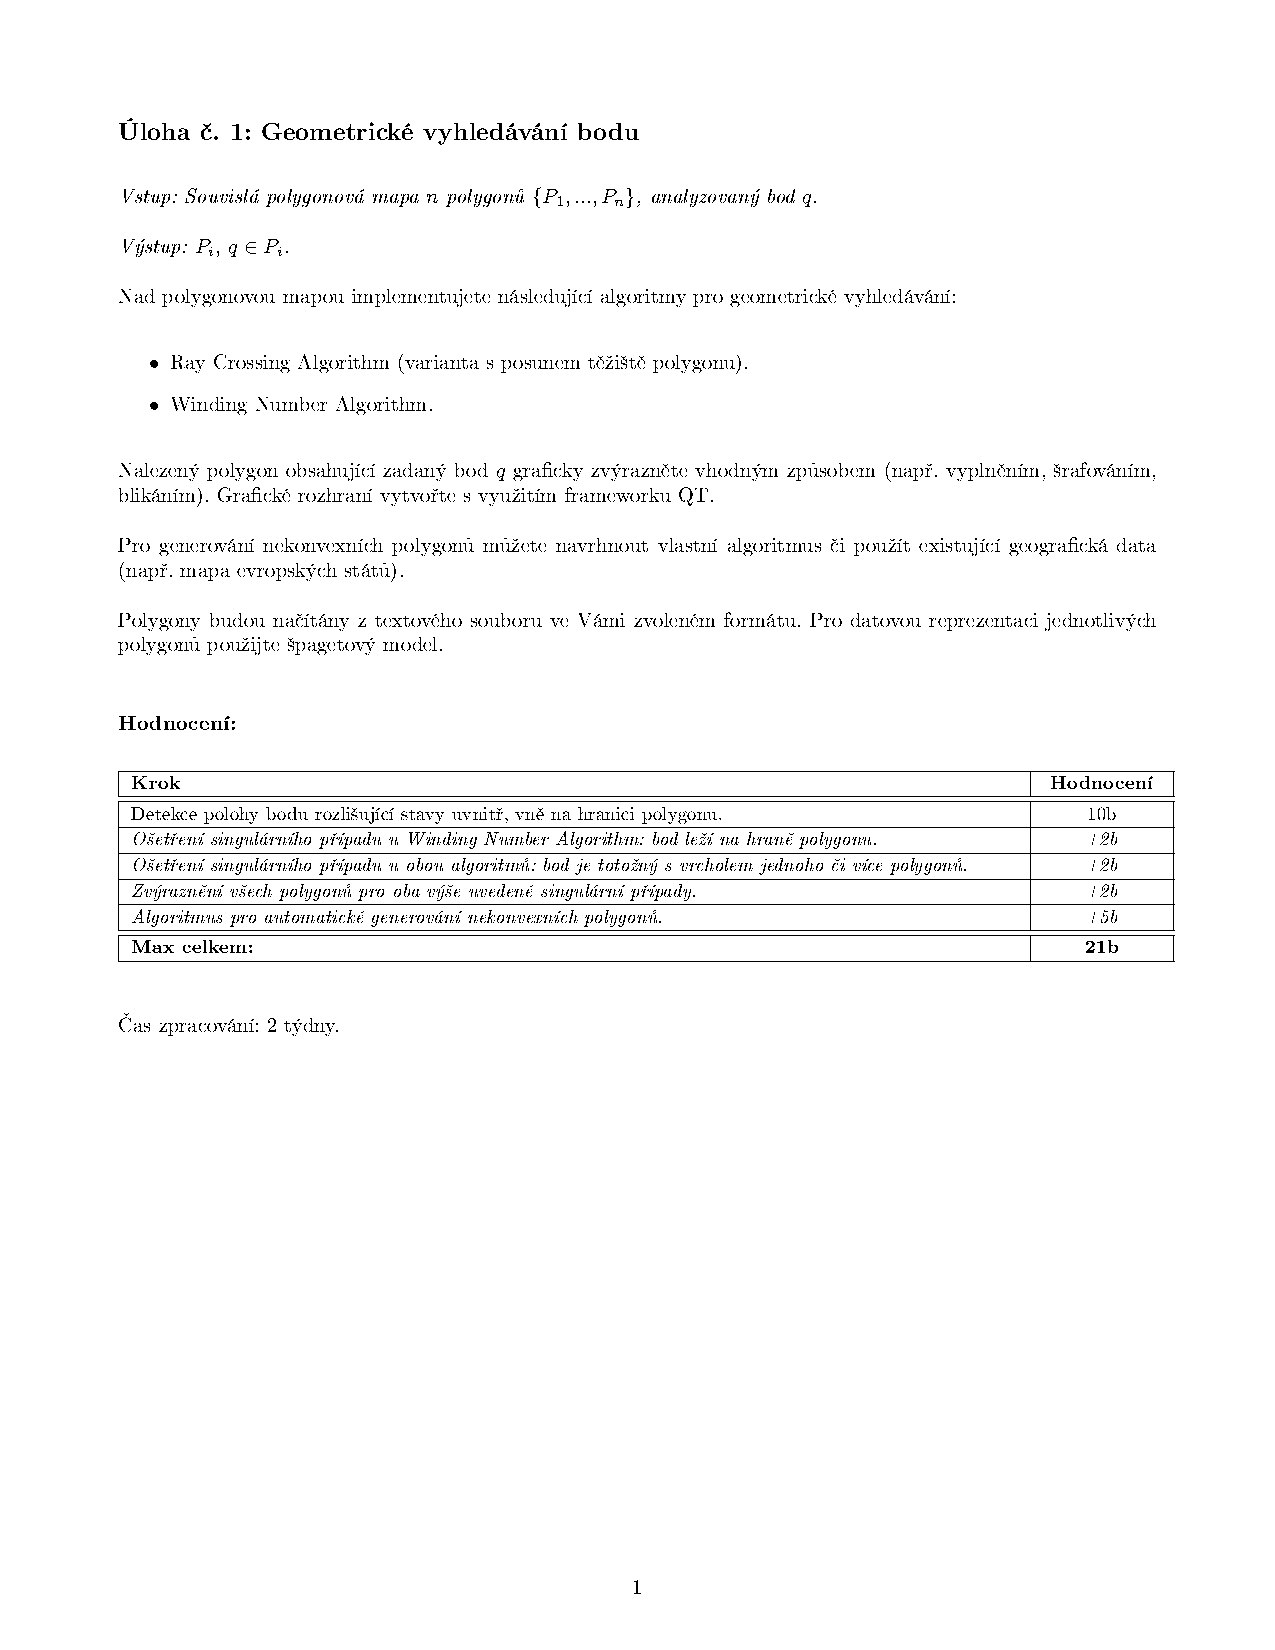
\includegraphics[clip, trim=0cm 10cm 0cm 3cm, width=1.2\textwidth]{zadani.pdf}
\end{figure}

\subsection{Údaje o bonusových úlohách}


\clearpage

\section{Popis a rozbor problému}
Hlavním cílem této úlohy je tvorba aplikace, která uživateli určí pozici zvoleného bodu q. Termínem pozice je myšlen polygon, kterému zadaný bod přísluší.
\\

V závislosti na tvaru polygonu rozlišujeme dva základní typy. Jedná se o konvexní a nekonvexní polygon. Polygon můžeme označit za konvexní právě tehdy, pokud jsou všechny vnitřní úhly konvexní, tedy v případě, že úhly jsou menší nebo rovny hodnotě 180 $^\circ$. Zároveň pro takový polygon platí, že všechny přímky, jejichž oba krajní body leží uvnitř polygonu, mají s tímto polygonem všechny body společné. Takový polygon, který není konvexní, lze označit jako nekonvexní či konkávní.
\\

Porovnání konvexního a nekonvexního objektu lze vidět na následujícím obrázku.
\begin{figure}[h]
	\centering
	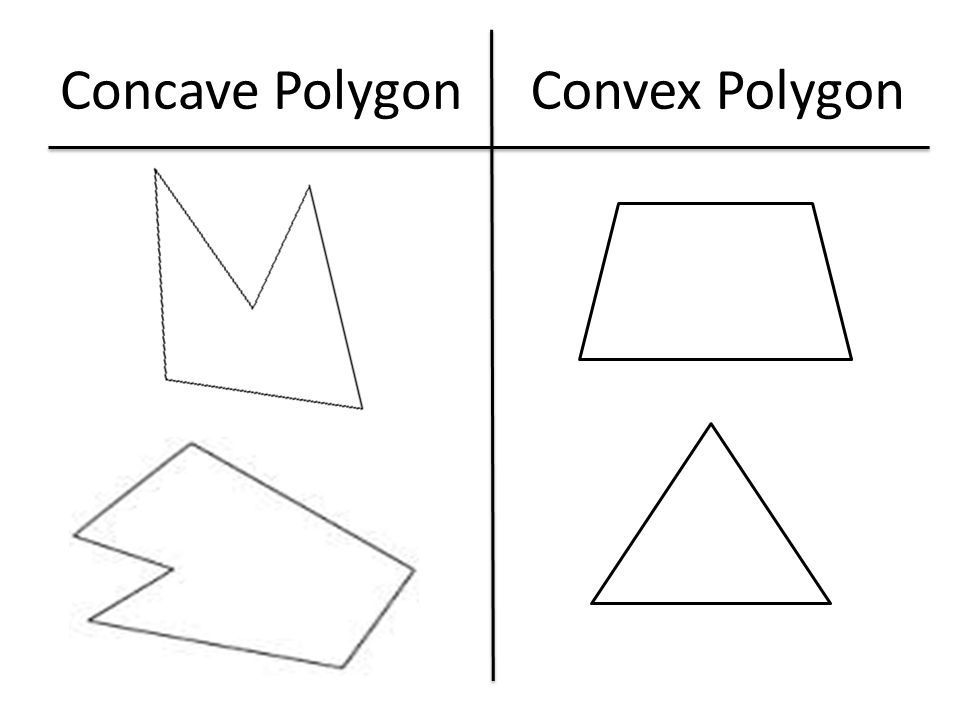
\includegraphics[width=10cm]{typy_polygonu.jpg}
	\caption{Porovnání konvexního a konkávního polygonu [zdroj: 1]}
\end{figure}

Bod q může mít vůči polygonu P jednu z těchto poloh:
\begin{enumerate}
\item Bod q leží uvnitř polygonu P.
\item Bod q leží vně polygonu P.
\item Bod q leží na hraně polygonu P.
\item Bod q je totožný s některým z vrcholu polygonu P.
\end{enumerate}


Pro určení pozice bodu q vůči polygonu existuje několik metod. V této aplikaci jsou implementován metody Ray Crossing Algorithm (varianta s posunem těžiště polygonu) a metoda Winding Number Algorithm.

\section{Popis použitých algoritmů}
Existuje mnoho metod pro určení pozice bodu q vůči polygonu P. Při volbě metod je vždy potřeba zhodnotit několik důležitých bodů, například požadavky vstupních/výstupních dat, časová náročnost či zda typ problému nespadá mezi NP problémy. V aplikaci byly použity algoritmy Ray Crossing Algorithm a Winding Number Algorithm. Mezi další známé metody pro určení pozice bodů patří třeba Line Sweep Algorithm (Zametací přímka), Divide and Conquer (Rozděl a panuj) či lze pozice určit i metodou hrubé síly (Brute Force Algorithm).

\subsection{Ray Crossing Algorithm}
Ray Crossing Algorithm lze do češtiny přeložit jako paprskový algoritmus. Primárně slouží k určení polohy bodu v konvexních mnohoúhelnících. Lze jej však zobecnit i pro nekonvexní. Obecně si lze metodu představit tak, že z libovolného bodu vedeme polopřímky a hodnotíme průsečíky přímky s hranami polygonu. \\

Označme si určovaný bod q. Z tohoto bodu je veden paprsek r (ray). Pokud si průsečík přímky r s hranami polygonu P označíme jako k, pak platí:
\begin{enumerate}
\item Pokud je k liché: Bod náleží polygonu P. $(q\in P)$ 
\item Pokud je k sudé: Bod nenáleží polygonu P.  $(q {\not \in} P)$ 
\end{enumerate}

\begin{figure}[h]
	\centering
	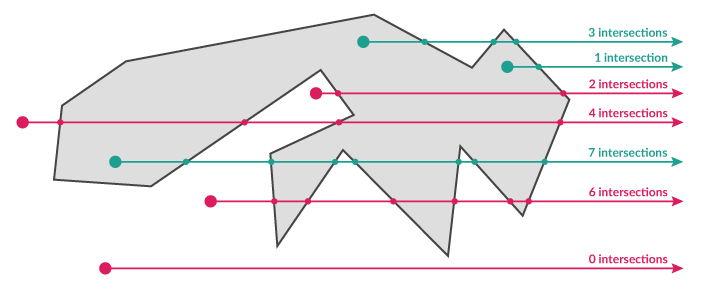
\includegraphics[width=10cm]{ray.png}
	\caption{Princip Ray Crossing Algorithm [zdroj: 2]}
\end{figure}

\subsubsection{Problematické situace}
Při použití Ray Crossing Algorithm může nastat několik problematických situací, které nelze opomenout. Tímto problémem jsou singularity. K singularitě v této metodě může dojít tehdy, pokud bod leží na hraně polygonu či pokud je bod totožný s některým z vrcholů polygonu. Z tohoto důvodu se využívá upravená varianta Ray Crossing Algorithm, kdy je provedena redukce souřadnic bodů 

\subsubsection{Implementace metody}
\begin{enumerate}
\item Nastavení počtu průsečíků rovno nule:  $ inters = 0 $ 
\item Redukce souřadnic x všech bodů polygonu vůči x-ové souřadnici bodu q:  $x'_i = x_i - x_q $ 
\item Redukce souřadnic y všech bodů polygonu vůči y-ové souřadnici bodu q:  $y'_i = y_i - y_q $ 
\item Volba podmínky:  $if(y'_i > 0)\&\&(y'_{i-1} <= 0)\|(y'_{i-1} > 0)\&\&(y'_{i} <= 0)  $ 
\item Při splnění podmínky:  $ x'_m = (x'_i y'_{i-1} - x'_{i-1} y'_i ) / (y'_i - y'_{i-1})$ 
\item Pokud $x'_m > 0$, zvýšení počtu průsečíků o jeden: $ inters = inters + 1 $
\item Určení zda počet průsečíků sudý či lichý: $if (inters\%2) = 0$, pak: $q\in P$ - počet průsečíků je sudý
\item V opačném případě: $q {\not \in} P$
\end{enumerate}

\subsection{Winding Number Algorithm}
Metoda ovíjení, či známá jako Winding Number Algorithm, je často používána pro určení pozice bodu vůči nekonvexnímu mnohoúhelníku. Algoritmus si lze představit tak, že se z určovaného bodu otáčíme postupně ke každému bodu polygonu a pokud se otáčíme po směru hodinových ručiček, úhel sčítáme, v opačném případě odčítáme. Pokud je výsledný úhel roven $2\pi$, lze říci, že bod náleží polygonu. V opačném případě nenáleží.

\begin{figure}[h]
	\centering
	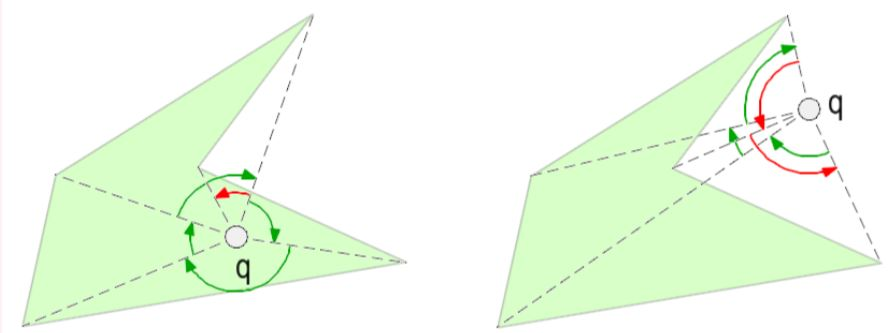
\includegraphics[width=10cm]{winding.jpg}
	\caption{Princip Winding Number Algorithm [zdroj: 3]}
\end{figure}

Při této metodě je zapotřebí si implementovat Winding Number $\Omega$. Pro $\Omega$ platí, že je rovna sumě všech rotací $\omega$ proti směru hodinových ručiček, které průvodič opíše nad všemi body: $ \Omega = \frac{1}{2\pi} \sum_{i=1}^n \omega_i^2$
\\
Orientace úhlů je dána:
\begin{enumerate}
\item Pokud je úhel $\sphericalangle p_i, q, p_{i+1}$ orientován ve směru hodinových ručiček, pak $\omega_i > 0$
\item Pokud je úhel $\sphericalangle p_i, q, p_{i+1}$ orientován proti směru hodinových ručiček, pak $\omega_i < 0$
\end{enumerate}


V závislosti na výsledné hodnotě $\Omega$ lze vyvodit následující závěry:
\begin{enumerate}
\item Pokud je $\Omega = 1$, pak platí $q \in P$ 
\item Pokud je $\Omega = 0$, pak platí $q { \not \in } P$
\end{enumerate}

\subsubsection{Problematické situace}
Pro Winding Number Algorithm je snadnější řešení singulárních případů. K těm dochází pouze v případě, že $q \approx p_i$.

\subsubsection{Implementace metody}
\begin{enumerate}
\item Nastavení výchozího úhlu $\omega$ rovno 0, volba tolerance $\epsilon$ : $\omega = 0, \epsilon = 1e-10$
\item Určení orientace $o_i$ bodu q ke straně $p_i, p_{i+1}$
\item Určení úhlu: $\omega_i = \sphericalangle p_i, q, p_{i+1}$
\item Volba podmínky - pokud pod vlevo: $\omega = \omega + \omega_i$
\item V opačném případě: $\omega = \omega - \omega_i$
\item Volba podmínky - pokud rozdíl: $(\omega - 2\pi) < \epsilon$, pak platí: $q \in P$
\item V opačném případě:  $ q { \not \in } P $
\end{enumerate}
\section{Vstupní data}


\section{Výstupní data}

\section{Aplikace}

\section{Dokumentace}

\clearpage
\section{Závěr}

\clearpage
\section{Reference}

\begin{enumerate}
\item  Presentation about convex and concave polygons [online][cit. 21.10.2018]. \\
Dostupné z: https://slideplayer.com/slide/6161031/  \\
\item  Introducing Wherewolf - A serverless boundary service from WNYC [online][cit. 21.10.2018]. \\
Dostupné z: https://source.opennews.org/articles/introducing-wherewolf/  \\
\item  BAYER, Tomáš. Geometrické vyhledávání [online][cit. 21.10.2018]. \\
Dostupné z: https://web.natur.cuni.cz/~bayertom/images/courses/Adk/adk3.pdf  \\

\end{enumerate}
\end{document}



 